% Канонический TikZ-рисунок варианта 17. Править только здесь.
\long\def\figStereoV17{%
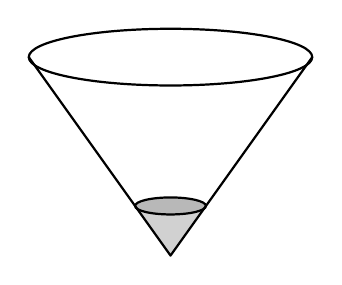
\begin{tikzpicture}[
  scale=0.9,
  line cap=round,
  line join=round
]
  \coordinate (S) at (0,-2.8);
  \coordinate (L) at (-2,0);
  \coordinate (R) at (2,0);

  % Точки на уровне жидкости:
  % высота малого конуса составляет 0,25 высоты большого
  \coordinate (A) at (-0.5,-2.1);
  \coordinate (B) at (0.5,-2.1);

  % Жидкость
  \fill[black!18]
    (S) --
    (A)
    arc[
      start angle=180,
      end angle=360,
      x radius=0.5,
      y radius=0.12
    ]
    -- cycle;

  \fill[black!28]
    (0,-2.1)
    ellipse[
      x radius=0.5,
      y radius=0.12
    ];

  % Сосуд
  \draw[thick]
    (0,0)
    ellipse[
      x radius=2,
      y radius=0.4
    ];

  \draw[thick]
    (L) -- (S) -- (R);

  % Поверхность жидкости
  \draw[thick]
    (0,-2.1)
    ellipse[
      x radius=0.5,
      y radius=0.12
    ];
\end{tikzpicture}
}
